% Compilar con: latexmk -lualatex -output-directory=out main.tex   (o `make pdf`)
\documentclass[11pt]{article}
% ---------------------------------------------------------------- idioma y fuentes (LuaLaTeX)
\usepackage[spanish,es-noshorthands]{babel}  % rótulo "Cuadro", como en el texto
\usepackage{fontspec}
\setmainfont{TeX Gyre Termes}
\usepackage{microtype}
\usepackage{csquotes}

% ---------------------------------------------------------------- página (límite: 10 páginas de cuerpo; referencias aparte)
\usepackage[a4paper,margin=2.2cm,top=2.2cm,bottom=2.2cm]{geometry}
\setlength{\emergencystretch}{1.5em}  % evita líneas desbordadas por cifras y macros que no se dividen
\usepackage{fancyhdr}
\setlength{\headheight}{12.2pt}
\pagestyle{fancy}\fancyhf{}
\rhead{\small Gestión de Derivados Financieros — Trabajo Calificado}
\lhead{\small PETROPERÚ S.A.}
\cfoot{\small \thepage\ de \pageref*{LastPage}}
\renewcommand{\headrulewidth}{0.4pt}
\usepackage{lastpage}
\usepackage[compact]{titlesec}
\titlespacing*{\section}{0pt}{1.0ex}{0.6ex}
\titlespacing*{\subsection}{0pt}{0.8ex}{0.4ex}
\usepackage{enumitem}\setlist{nosep,leftmargin=*}
\setlength{\parskip}{0.3em}\setlength{\parindent}{0pt}

% ---------------------------------------------------------------- matemática, tablas, figuras
\usepackage{amsmath,amssymb}
\usepackage{booktabs,tabularx,multirow}
\usepackage{graphicx}
\graphicspath{{generado/figuras/}{figuras/}}
\usepackage[font=small,labelfont=bf,skip=3pt]{caption}
\usepackage{float}
\usepackage{xcolor}
\usepackage{colortbl}   % bandas sombreadas en cuadros (p. ej., matriz de riesgos)
\usepackage{array}
\colorlet{prioAlta}{red!13}\colorlet{prioMedia}{orange!18}\colorlet{prioNo}{gray!12}  % prioridades de riesgo
\usepackage{tikz}
\usetikzlibrary{positioning,arrows.meta}

% Nota de fuente OBLIGATORIA bajo cada tabla/figura (criterio "Material de apoyo").
\newcommand{\fuente}[1]{\par\vspace{2pt}{\footnotesize\raggedright\textit{Fuente:} #1\par}}

% ---------------------------------------------------------------- bibliografía (APA 7)
\usepackage[backend=biber,style=apa]{biblatex}
\addbibresource{referencias.bib}
\renewcommand*{\bibfont}{\small}\setlength{\bibitemsep}{0pt}   % referencias en letra menor (ahorra espacio para el límite de 10 p.)

\usepackage[hidelinks]{hyperref}

% ---------------------------------------------------------------- cifras generadas (NO escribir números a mano)
\IfFileExists{generado/valores.tex}{% ARCHIVO GENERADO por scripts/run_all.py — NO EDITAR A MANO

\newcommand{\ApreciacionSolDiez}{11.1\,\%}
\newcommand{\BNCuota}{17.0}
\newcommand{\BNCuotaAmort}{218.3}
\newcommand{\BNCuotaNominal}{218.5}
\newcommand{\BNCuotasAmort}{18}
\newcommand{\BNCuotasPagadas}{9}
\newcommand{\BNCuotasRem}{27}
\newcommand{\BNCuotasTot}{46}
\newcommand{\BNMesesGracia}{18}
\newcommand{\BNSaldoJunio}{3,765.6}
\newcommand{\BNSaldoPEN}{3,765.6}
\newcommand{\BNSaldoRem}{3,765.6}
\newcommand{\BNSaldoUSD}{1,118.0}
\newcommand{\BNTasa}{5.55\,\%}
\newcommand{\Backwardation}{6.5\,\%}
\newcommand{\BonosDVCien}{166}
\newcommand{\BonosDurMod}{8.2}
\newcommand{\BonosLibros}{3,096.0}
\newcommand{\BonosLibrosNotaA}{3,107.0}
\newcommand{\BonosNominal}{3,000}
\newcommand{\BonosVR}{2,030.3}
\newcommand{\BrentFut}{105.28}
\newcommand{\BrentWTI}{12.7}
\newcommand{\CCSCVAUSD}{1.7}
\newcommand{\CCSCVApb}{11}
\newcommand{\CCSCuotaUSD}{5.2}
\newcommand{\CCSEPEMax}{23.9}
\newcommand{\CCSNocionalMax}{1,095.7}
\newcommand{\CCSNocionalMin}{1,095.7}
\newcommand{\CCSNocionalUSD}{1,095.7}
\newcommand{\CCSTasaAllIn}{5.98\,\%}
\newcommand{\CCSTasaMax}{6.01\,\%}
\newcommand{\CCSTasaMin}{5.82\,\%}
\newcommand{\CCSTasaSBS}{5.92\,\%}
\newcommand{\CCSTasaUSD}{5.87\,\%}
\newcommand{\CCSTotalUSD}{1,192.9}
\newcommand{\CCSVPPataPEN}{1,116.9}
\newcommand{\CCSValMasDiez}{101.9}
\newcommand{\CCSValMenosDiez}{123.7}
\newcommand{\CCSVsBN}{32}
\newcommand{\CESCELibros}{705.3}
\newcommand{\CESCESaldo}{722.2}
\newcommand{\CESCETasa}{3.285\,\%}
\newcommand{\CapTrabajoVeinticinco}{(2,296.4)}
\newcommand{\CoberturaCrudoPct}{80\,\%}
\newcommand{\CoberturaFX}{96\,\%}
\newcommand{\ColateralConjunto}{172.9}
\newcommand{\ColateralTC}{121.2}
\newcommand{\ColateralWTI}{51.8}
\newcommand{\CollarCall}{98.05}
\newcommand{\CollarCallVolBaja}{97.17}
\newcommand{\CollarCallVolMedia}{97.58}
\newcommand{\CollarCallsCapas}{103.68 / 100.38 / 98.05}
\newcommand{\CollarPut}{77.90}
\newcommand{\CollarPutsCapas}{83.30 / 80.10 / 77.90}
\newcommand{\CollarValMasDiez}{5.8}
\newcommand{\CollarValMenosDiez}{5.7}
\newcommand{\ComprasMBDC}{87}
\newcommand{\ComprasUSD}{2,490.0}
\newcommand{\ContratosEquiv}{2,321}
\newcommand{\ContratosH}{2,347}
\newcommand{\ContratosHBrent}{2,648}
\newcommand{\ConvenienciaImplicita}{44.7\,\%}
\newcommand{\CostoPutTotal}{7.2}
\newcommand{\CostoSwap}{3.7}
\newcommand{\CuponCuarentaSiete}{5.625\,\%}
\newcommand{\CuponTreintaDos}{4.750\,\%}
\newcommand{\DUCrisis}{N.°~003-2026}
\newcommand{\DUCrisisMonto}{2,000}
\newcommand{\DeficitConjunto}{150.7}
\newcommand{\DeltaPutAbs}{0.25}
\newcommand{\DeudaTotal}{6,429.0}
\newcommand{\DifCambioBN}{119.3}
\newcommand{\EfectividadBrent}{79\,\%}
\newcommand{\EfectividadWTI}{99\,\%}
\newcommand{\EscConCobMenosDiez}{6.1}
\newcommand{\EscSinCobMenosDiez}{152.0}
\newcommand{\EurNeto}{95.6}
\newcommand{\FEPCpct}{0.43\,\%}
\newcommand{\FechaValorizacion}{28 de setiembre de 2026}
\newcommand{\FwdSwapRate}{4.85\,\%}
\newcommand{\GananciaDifCambio}{13.4}
\newcommand{\GananciaInvHoy}{102.1}
\newcommand{\GananciaMaxCollar}{34.9}
\newcommand{\GananciaMaxMixto}{21.8}
\newcommand{\HistDesde}{ene-2021}
\newcommand{\HistHasta}{ago-2026}
\newcommand{\IngresosVeinticinco}{3,380.4}
\newcommand{\IngresosVeinticuatro}{3,456.4}
\newcommand{\InsumosPendientes}{0}
\newcommand{\InvCrudoMMbl}{2.901}
\newcommand{\InvCrudoMbl}{2,901}
\newcommand{\InvCrudoUSD}{168.4}
\newcommand{\InvCubiertoMMbl}{2.32}
\newcommand{\InvCubiertoValor}{214.9}
\newcommand{\InvHidroUSD}{563.5}
\newcommand{\InvRefinadosUSD}{313.5}
\newcommand{\InvValorHoy}{268.6}
\newcommand{\JpyNeto}{50.5}
\newcommand{\LGD}{60\,\%}
\newcommand{\LimiteCrudo}{50\,\%--80\,\%}
\newcommand{\LimiteFX}{70\,\%--100\,\%}
\newcommand{\LineasLibres}{22.2}
\newcommand{\LineasPct}{94\,\%}
\newcommand{\LineasRev}{376.9}
\newcommand{\LineasUsadas}{354.6}
\newcommand{\NCapas}{3}
\newcommand{\NDFCostoAnual}{0.24\,\%}
\newcommand{\NDFCostoUSD}{0.13}
\newcommand{\NDFDias}{91}
\newcommand{\NDFDifSBSPips}{0.6}
\newcommand{\NDFForward}{3.4347}
\newcommand{\NDFForwardSBS}{3.4346}
\newcommand{\NDFNocional}{750.7}
\newcommand{\NDFPct}{80\,\%}
\newcommand{\NDFPuntos}{(20.5)}
\newcommand{\NDFValMasDiez}{19.7}
\newcommand{\NDFValMenosDiez}{24.0}
\newcommand{\PENDosAnios}{4.52\,\%}
\newcommand{\PENTresAnios}{5.03\,\%}
\newcommand{\PENTresMeses}{3.90\,\%}
\newcommand{\PENUnAnio}{3.97\,\%}
\newcommand{\PenNeto}{(4,704.0)}
\newcommand{\PenNetoAbs}{4,704.0}
\newcommand{\PenNetoCrec}{21\,\%}
\newcommand{\PenNetoUSD}{1,397}
\newcommand{\PenNetoVeinticuatro}{3,880.1}
\newcommand{\PenOtrosPasFin}{3,824.5}
\newcommand{\PerdidaInvVeinte}{33.3}
\newcommand{\PerdidaInvVeinteXUB}{2.3}
\newcommand{\PerdidaMaxCollar}{44.4}
\newcommand{\PerdidaMaxMixto}{34.0}
\newcommand{\PerdidaSinCobForward}{17.6}
\newcommand{\PerdidaSinCobTreinta}{80.6}
\newcommand{\PerdidaVeinticinco}{(601.5)}
\newcommand{\PerdidaVeinticincoAbs}{601.5}
\newcommand{\PerdidaVeinticuatro}{(773.9)}
\newcommand{\PlazoDiasCapas}{17 / 50 / 79}
\newcommand{\PlazoDiasOpc}{79}
\newcommand{\PlazoMeses}{3}
\newcommand{\PosicionHoy}{4,704.0}
\newcommand{\PrecioCompras}{78.66}
\newcommand{\PrestamoPuente}{475}
\newcommand{\PrimaPut}{3.12}
\newcommand{\PutPctFwd}{90\,\%}
\newcommand{\RUSDCont}{4.12\,\%}
\newcommand{\RatioH}{1.01}
\newcommand{\RatioHBrent}{1.14}
\newcommand{\ReduccionFX}{96\,\%}
\newcommand{\RepartoCollar}{50\,\%}
\newcommand{\RepartoSwap}{50\,\%}
\newcommand{\ResiduoTotal}{187.7}
\newcommand{\RestoPEN}{938.4}
\newcommand{\RotacionDias}{33}
\newcommand{\SemanasH}{101}
\newcommand{\SensApreciacion}{155.2}
\newcommand{\SensDepreciacion}{127.0}
\newcommand{\SensibilidadFX}{139.7}
\newcommand{\SpotAsk}{3.4390}
\newcommand{\SpotBid}{3.4367}
\newcommand{\SpotUSDPEN}{3.4379}
\newcommand{\SpreadBonosPb}{569}
\newcommand{\SwapCiti}{14.6}
\newcommand{\SwapCitiJunio}{5.9}
\newcommand{\SwapPrecio}{89.38}
\newcommand{\SwapValDiez}{10.3}
\newcommand{\TCcierre}{3.367}
\newcommand{\TCcierreBCRPVeinticinco}{3.361}
\newcommand{\TCcierreBCRPVeinticuatro}{3.765}
\newcommand{\TCvarVeinticinco}{-10.7\,\%}
\newcommand{\USDCincoAnios}{4.80\,\%}
\newcommand{\USDDosAnios}{4.72\,\%}
\newcommand{\USDTresAnios}{4.80\,\%}
\newcommand{\USDTresMeses}{4.14\,\%}
\newcommand{\USDTresMesesSimple}{4.08\,\%}
\newcommand{\USDUnAnio}{4.50\,\%}
\newcommand{\USTDurDic}{4.04\,\%}
\newcommand{\UmbralNecesario}{151}
\newcommand{\UtilidadBruta}{14.4}
\newcommand{\VaRCrudoCon}{36.5}
\newcommand{\VaRCrudoSin}{93.3}
\newcommand{\VaRFXCon}{3.1}
\newcommand{\VaRFXSin}{78.5}
\newcommand{\VegaCollar}{(0.01)}
\newcommand{\VencMenosUnAnio}{3,163.4}
\newcommand{\VolCrudo}{56.1\,\%}
\newcommand{\VolHistTC}{5.6\,\%}
\newcommand{\VolHistWTI}{29.3\,\%}
\newcommand{\VolRealCL}{55.8\,\%}
\newcommand{\VolSensBaja}{35\,\%}
\newcommand{\VolSensMedia}{45\,\%}
\newcommand{\VolTC}{6.75\,\%}
\newcommand{\WTIFut}{86.54}
\newcommand{\WTIFutDoce}{76.03}
\newcommand{\WTIFutDos}{89.01}
\newcommand{\WTIFutUno}{92.60}
\newcommand{\WTISpot}{92.60}
\newcommand{\WTIcierreVeinticinco}{57.42}
\newcommand{\WTIcierreVeinticuatro}{71.72}
\newcommand{\WTIvarVeinticinco}{-19.9\,\%}
\newcommand{\YTMBonos}{9.7\,\%}
}{%
  \PackageWarning{informe}{Falta generado/valores.tex: ejecute 'make calc'}}

% Marca visible para lo pendiente (el hook y 'make final' fallan si queda alguna)
\newcommand{\pendiente}[1]{\textcolor{red}{\textbf{[PENDIENTE: #1]}}}


\begin{document}

% Portada COMPACTA (la portada cuenta dentro de las 10 páginas)
\begin{center}
  {\small Universidad del Pacífico — Maestría en Finanzas — Gestión de Derivados Financieros (Prof. Alberto Humala)}\\[4pt]
  {\Large\bfseries Gestión de riesgos financieros de PETROPERÚ S.A.\\ mediante instrumentos derivados}\\[4pt]
  {\small Informe a la Gerencia General — Gerencia de Finanzas}\\[2pt]
  {\small Grupo: Luis Ramírez Osorio, Sabino Sifuentes Motta, Jesús Quinte Sánchez y Evelyn Mendoza Rosales \quad Lima, 5 de octubre de 2026}
\end{center}
\vspace{-0.5em}

% Presupuesto de páginas (total 10). Puntaje de la rúbrica entre corchetes.
% [1.5 pts] ~0.8 páginas. Qué es la empresa, por qué importa, objetivo del informe.
% Cifras solo con macros de generado/valores.tex.
\section{Introducción y objetivo}

PETROPERÚ es la empresa estatal que refina y comercializa combustibles en el Perú: opera la Nueva Refinería
Talara (NRT), las refinerías de Iquitos y Conchán y el Oleoducto Norperuano. Reporta a la SMV y su moneda
funcional es el dólar estadounidense. En 2025 registró ingresos por US\$~\IngresosVeinticinco\ millones,
una pérdida neta de US\$~\PerdidaVeinticincoAbs\ millones y un capital de trabajo de US\$~\CapTrabajoVeinticinco\ millones;
el auditor incluyó una incertidumbre material sobre la continuidad como empresa en marcha
(Cuadro~\ref{tab:indicadores}) \parencite{petroperu2026eeff}. La calificación internacional sigue en grado
especulativo: S\&P la rebajó a B- en diciembre de 2025 y la reafirmó en mayo de 2026 con perspectiva negativa;
Moody's la reafirmó en Caa1 en setiembre de 2026 y cambió su perspectiva a positiva, y Fitch retiró sus calificaciones
en enero de 2026 \parencite{sp2026petroperu,moodys2026petroperu,petroperu2026clasif}.

En este contexto la volatilidad de mercado ya no es un tema secundario: cada dólar que se pierde por tipo de cambio
o por el precio del crudo reduce una liquidez escasa \parencite{froot1993}. La Nota~3 confirma que la Compañía
no usa derivados para cubrir el riesgo cambiario y asume ese riesgo; el único derivado revelado son swaps de monedas
de corto plazo con Citibank (activo de US\$~\SwapCiti\ millones, Nota~9(g)), sin una política de cobertura
que los enmarque. El precio del crudo tampoco se cubre: solo se amortigua en parte con el Fondo de Estabilización
de Precios (FEPC).

\textbf{Objetivo.} Sustentar ante la Gerencia General el uso de instrumentos derivados para gestionar los riesgos
financieros del negocio. Para ello: (i) se identifican y cuantifican los riesgos con los estados financieros
auditados 2025; (ii) se diseñan y valorizan dos estrategias con uso intensivo de derivados, un \emph{cross currency
swap} (CCS) con forwards sin entrega (NDF) para el riesgo cambiario y un swap y un collar de opciones sobre WTI para
el precio del crudo; y (iii) se proponen las condiciones de implementación. Las exposiciones corresponden al cierre
de 2025 y los precios de mercado al \FechaValorizacion, fecha de valorización de este informe.

% ARCHIVO GENERADO — NO EDITAR A MANO
\begin{table}[htbp]\centering\small
\caption{Indicadores financieros de PETROPERÚ (US\$ millones)}\label{tab:indicadores}
\begin{tabular}{lrrr}
\toprule
 & \textbf{2024} & \textbf{2025} & \textbf{Comentario} \\
\midrule
Ingresos de actividades ordinarias & 3,456.4 & 3,380.4 & Menor precio del crudo \\
Resultado neto & (773.9) & (601.5) & Pérdida menor que en 2024 \\
Capital de trabajo & (1,900.0) & (2,296.4) & Pasivo corriente > activo corriente \\
Otros pasivos financieros & 5,610.7 & 5,168.8 & 100\% a tasa fija \\
Deuda neta / capital total & 0.70 & 0.78 & Mayor apalancamiento \\
\bottomrule
\end{tabular}
\fuente{PETROPERÚ, EEFF auditados al 31.12.2025 (Gaveglio, Aparicio y Asociados, 2026), Notas 1, 3, 5 y 14. Elaboración propia.}
\end{table}

      % 0.6 p  [1.5]
% [4 pts] ~2.6 páginas. Identificación y CUANTIFICACIÓN de riesgos con cita a Nota/página.
% Estructura por riesgo: fuente (qué partida) → dirección (qué movimiento daña) → magnitud → coberturas naturales.
\section{Identificación de riesgos financieros}

La Nota 3.1 clasifica la exposición de PETROPERÚ en riesgos de mercado (tipo de cambio, tasa de interés y precio
del crudo), de crédito y de liquidez. El Cuadro~\ref{tab:matriz} resume su magnitud y si pueden gestionarse
eficientemente con derivados.

\begin{table}[htbp]\centering\small
\caption{Matriz de riesgos financieros de PETROPERÚ al cierre de 2025}\label{tab:matriz}
\newcommand{\muestra}[1]{\fcolorbox{gray!60}{#1}{\rule{0pt}{0.55em}\rule{0.9em}{0pt}}}
\renewcommand{\arraystretch}{1.25}
\setlength{\fboxsep}{0pt}
\newcommand{\sep}{\arrayrulecolor{white}\specialrule{1.2pt}{0pt}{0pt}\arrayrulecolor{black}}
\begin{tabularx}{\linewidth}{>{\raggedright\arraybackslash\bfseries}p{1.85cm}
    >{\raggedright\arraybackslash}X
    >{\raggedright\arraybackslash}p{3.0cm}
    >{\raggedright\arraybackslash}p{3.45cm}
    >{\raggedright\arraybackslash}p{3.0cm}}
\toprule
\normalfont\textbf{Riesgo} & \textbf{Origen} & \textbf{Exposición} & \textbf{Impacto (US\$ MM)} & \textbf{Respuesta} \\
\midrule
\rowcolor{prioAlta}
Tipo de cambio & Pasivo neto en S/: préstamo del Banco de la Nación (BN) y cuentas por pagar
  & S/~\PenNetoAbs\ MM \newline (US\$~\PenNetoUSD\ MM)
  & TC $-10$\,\%: (\SensApreciacion) \newline TC $+10$\,\%: \SensDepreciacion
  & CCS + NDF \newline (Estrategia 1) \\ \sep
\rowcolor{prioAlta}
Precio del crudo & Inventario de crudo; compras de \ComprasMBDC\ MBDC
  & \InvCrudoMbl\ MBL \newline (US\$~\InvCrudoUSD\ MM)
  & WTI $-20$\,\%: (\PerdidaInvVeinte) \newline = \PerdidaInvVeinteXUB\ veces la utilidad bruta
  & Swap o collar OTC \newline (Estrategia 2) \\ \sep
\rowcolor{prioMedia}
Tasa de interés & Bonos a tasa fija; refinanciación del CESCE y de líneas de corto plazo
  & Bonos: US\$~\BonosVR\ MM a mercado \newline (US\$~\BonosLibros\ MM en libros)
  & $\pm100$~pb: $\mp$\BonosDVCien\ en el valor razonable
  & Solo la tasa base, no el spread \\ \sep
\rowcolor{prioNo}
Liquidez & Capital de trabajo negativo; líneas usadas al \LineasPct
  & US\$~\VencMenosUnAnio\ MM de pagos a menos de un año
  & Restricción, no riesgo de precio
  & Condiciona el diseño: sin márgenes ni primas altas \\ \sep
\rowcolor{prioNo}
Crédito & Mayoristas y entidades del Estado
  & Baja concentración (Nota 3.1(b))
  & No significativo
  & No es necesario \\
\bottomrule
\end{tabularx}
\par\vspace{3pt}{\footnotesize\raggedright\textbf{Prioridad:}\quad
  \muestra{prioAlta}~Alta: se cubre con derivados\qquad
  \muestra{prioMedia}~Media: cobertura parcial\qquad
  \muestra{prioNo}~No se cubre con derivados\par}
\fuente{\textcite{petroperu2026eeff}, Notas 3, 10 y 14 (pp.~42--46, 60--61 y 74--78). Elaboración propia.}
\end{table}

\subsection{Riesgo de tipo de cambio}
Con contabilidad en dólares, el riesgo surge de las partidas en soles, euros y yenes. La exposición relevante es en
soles: una posición pasiva neta de S/~\PenNetoAbs\ millones (US\$~\PenNetoUSD\ millones al TC SBS de \TCcierre\ que usa el EEFF),
\PenNetoCrec\ mayor que la de 2024 (S/~\PenNetoVeinticuatro\ millones). La concentra el rubro \emph{otros pasivos
financieros} (S/~\PenOtrosPasFin\ millones), que incluye el préstamo del BN con garantía soberana por
S/~\BNSaldoPEN\ millones al \BNTasa, pagadero en \BNCuotasTot\ cuotas mensuales de enero de 2025 a diciembre de 2028
(Nota~14(ii), p.~74); como en 2025 solo se pagaron intereses, la sección~3 supone \BNCuotasSup\ cuotas desde 2026. Las posiciones en euros (activa por EUR~\EurNeto\ millones) y yenes (pasiva por
JPY~\JpyNeto\ millones) no son significativas según la Gerencia (Figura~\ref{fig:posicion}).

\begin{figure}[htbp]\centering
  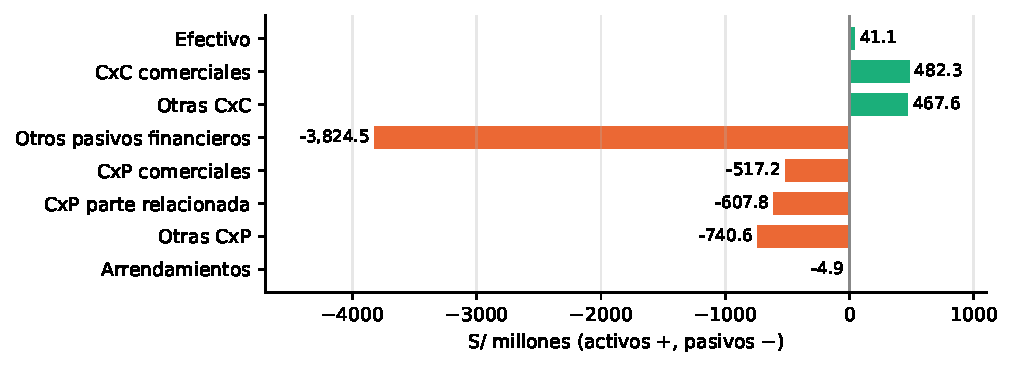
\includegraphics[width=0.86\linewidth]{f_posicion_pen}
  \caption{Composición de la posición en soles al cierre de 2025 (S/ millones)}\label{fig:posicion}
  \fuente{\textcite{petroperu2026eeff}, Nota 3.1(a)(i), p.~42. Elaboración propia.}
\end{figure}

El riesgo ya se materializó: en 2025 el tipo de cambio interbancario medio del BCRP pasó de \TCcierreBCRPVeinticuatro\ a
\TCcierreBCRPVeinticinco\ (\TCvarVeinticinco; el sol se apreció, Figura~\ref{fig:historia}) y la diferencia de
cambio aumentó en US\$~\DifCambioBN\ millones el saldo en dólares del préstamo del BN (Nota~14(c), p.~77), aunque en
el agregado la Compañía reportó una ganancia cambiaria neta de US\$~\GananciaDifCambio\ millones. La Compañía estima
que un movimiento de $\pm$10\,\% del dólar frente al sol afecta el resultado antes de impuestos en
$\pm$US\$~\SensibilidadFX\ millones, una aproximación lineal. El cálculo exacto es asimétrico: $-$US\$~\SensApreciacion\
millones si el TC cae 10\,\% y +US\$~\SensDepreciacion\ millones si sube 10\,\%. El descalce no es solo contable: las ventas
locales se facturan en soles, pero sus precios siguen la paridad de importación en dólares (Nota~1-c), por lo que
económicamente son flujos en dólares que no cubren de forma natural una deuda en soles a tasa fija.

\begin{figure}[htbp]\centering
  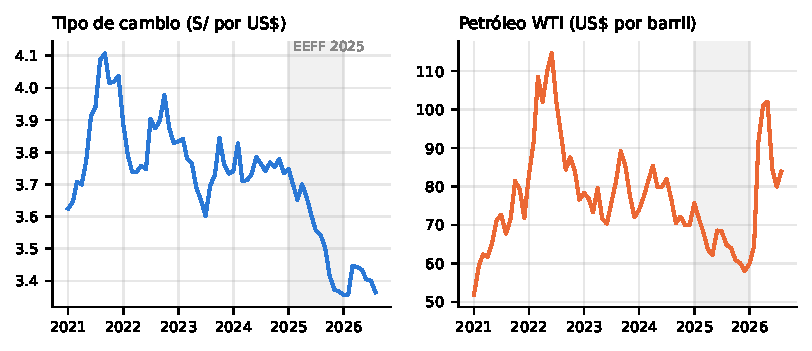
\includegraphics[width=0.9\linewidth]{f_historia}
  \caption{Tipo de cambio y precio del WTI, promedios mensuales (\HistDesde\ a \HistHasta)}\label{fig:historia}
  \fuente{\textcite{bcrpseries2026}, series PN01210PM y PN01660XM. Volatilidad anualizada de los retornos
  logarítmicos mensuales: TC \VolHistTC; WTI \VolHistWTI. Elaboración propia.}
\end{figure}

\subsection{Riesgo de precio del crudo}
Es el riesgo operativo-financiero más directo. En 2025 PETROPERÚ compró crudo y productos por
US\$~\ComprasUSD\ millones, a un precio promedio de US\$~\PrecioCompras/bl y con un volumen de \ComprasMBDC\ MBDC
(Nota~23, p.~93), pero el crudo cerró el año en US\$~\WTIcierreVeinticinco/bl, \WTIvarVeinticinco\ frente a los
US\$~\WTIcierreVeinticuatro/bl de 2024 (Nota~10, p.~61). Entre la compra y la venta del producto refinado pasan
varias semanas, y en ese lapso el inventario pierde valor si el precio cae; la Nota~1-d señala esta caída como una
causa de la pérdida de 2025. Al cierre, el inventario de crudo era de \InvCrudoMbl\ MBL (US\$~\InvCrudoUSD\ millones)
y el de hidrocarburos sumaba US\$~\InvHidroUSD\ millones. Con una utilidad bruta de apenas
US\$~\UtilidadBruta\ millones, una caída de 20\,\% del WTI sobre el inventario de crudo (US\$~\PerdidaInvVeinte\
millones) equivale a \PerdidaInvVeinteXUB\ veces la utilidad bruta del año. El riesgo es simétrico y de gran escala:
en 2026 el WTI subió hasta US\$~\WTISpot/bl al \FechaValorizacion, en plena crisis de oferta en Medio Oriente
\parencite{reuters2026oil}. El FEPC solo alcanza al Diésel BX y al Petróleo Industrial~6 y en 2025 fue un aporte
neto (\FEPCpct\ de los ingresos), no una compensación (Nota~1-c, p.~19).

\subsection{Riesgos de tasa de interés, liquidez y crédito}
Toda la deuda está pactada a tasa fija (Figura~\ref{fig:deuda}): bonos 2032 (\CuponTreintaDos) y 2047 (\CuponCuarentaSiete) por
US\$~\BonosNominal\ millones nominales, el préstamo CESCE (\CESCETasa, 2030), el préstamo del BN y líneas de corto
plazo. No hay riesgo de flujo de caja por tasas variables; el riesgo está en el valor razonable y en la
refinanciación. Los bonos valen US\$~\BonosVR\ millones a mercado frente a US\$~\BonosLibros\ millones en libros
(Nota~14(d), p.~78), lo que implica un rendimiento de \YTMBonos\ (cálculo propio): un spread de crédito de unos
\SpreadBonosPb~pb sobre el Tesoro de EE.\,UU. de igual duración (\USTDurDic). Con una duración modificada de \BonosDurMod\ años, cada 100~pb modifican su valor en unos
US\$~\BonosDVCien\ millones. Además, por la opinión con salvedades se incumplió un covenant no financiero del CESCE y su
saldo (US\$~\CESCESaldo\ millones) se reclasificó al corto plazo. Un swap puede fijar la tasa base, pero no el spread,
que es el componente dominante.

\begin{figure}[htbp]\centering
  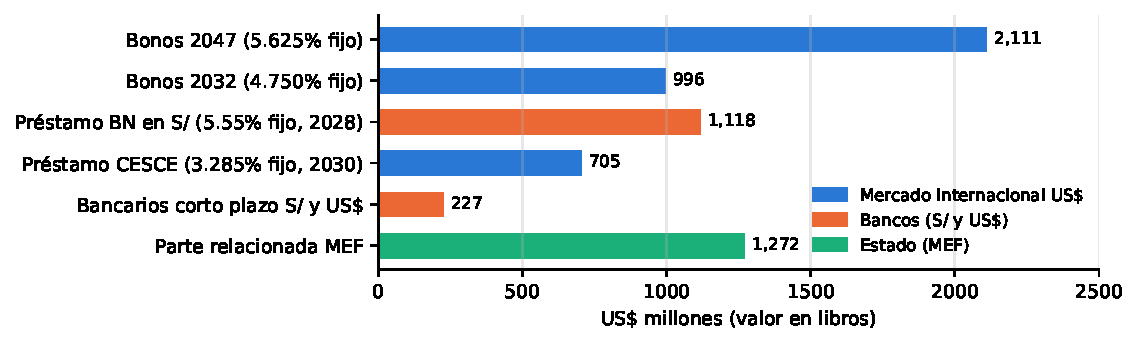
\includegraphics[width=0.86\linewidth]{f_deuda}
  \caption{Deuda financiera y con el accionista al cierre de 2025 (US\$~\DeudaTotal\ millones, sin intereses devengados)}\label{fig:deuda}
  \fuente{\textcite{petroperu2026eeff}, Nota 14(a), p.~76, y Nota 3.2, p.~46. Elaboración propia.}
\end{figure}

El riesgo de liquidez es crítico: de US\$~\LineasRev\ millones en líneas revolventes se usaban
US\$~\LineasUsadas\ millones (\LineasPct), y los pagos no descontados a menos de un año suman
US\$~\VencMenosUnAnio\ millones (Nota 3.1(c), pp.~44--45). No se cubre con derivados, pero condiciona su diseño:
deben evitarse instrumentos con llamadas de margen diarias, como los futuros en bolsa, y primas iniciales altas.
El riesgo de crédito es bajo, porque la cartera se concentra en mayoristas de primer nivel y entidades del Estado.
           % 2.0 p  [4.0]
% [4 + 4 pts] ~4 páginas. Dos estrategias con uso INTENSIVO de derivados: diseño, valorización y escenarios.
% Tablas y figuras SOLO desde generado/ (make calc) o con macros. Cada una con \fuente{...}.
\section{Estrategias de cobertura con instrumentos derivados}

\subsection{Estrategia 1: \emph{cross currency swap} y NDF para el riesgo cambiario}

\textbf{Diseño.} Se propone un CCS amortizable con un banco de primer nivel que replique el cronograma remanente del
préstamo del BN. PETROPERÚ \textbf{recibe} cada mes, en soles, la cuota del préstamo y
\textbf{paga} una cuota en dólares a tasa fija sobre un nocional de US\$~\CCSNocionalUSD\ millones. Así la deuda en
soles se convierte sintéticamente en deuda en la moneda funcional (Figura~\ref{fig:ccs}). El resto de la posición en
soles (S/~\RestoPEN\ millones, sobre todo cuentas por pagar) se cubre en un \NDFPct\ con NDF de compra de soles a
\NDFDias\ días, renovables, que se liquidan por diferencias en dólares sin entregar el principal. Esa posición usa
saldos de diciembre de 2025 (salvo el BN) y debe actualizarse antes de pactar; los swaps de corto plazo con Citibank
siguen vigentes (activo de US\$~\SwapCitiJunio\ millones a junio de 2026) sin que se revele su nocional, que debe
restarse del NDF si cubre soles. El EEFF no publica el cronograma del BN (\BNCuotasTot\ cuotas en 48 meses), pero a
junio de 2026 el saldo seguía en S/~\BNSaldoJunio\ millones y era íntegramente no corriente
\parencite{petroperu2026eeffjun}: no vence principal antes de julio de 2027. Se supone que se pagan solo
intereses hasta junio de 2027 (S/~\BNCuota\ millones al mes) y luego \BNCuotasAmort\ cuotas francesas de
S/~\BNCuotaAmort\ millones, con la TEA llevada a tasa mensual, $(1+\text{TEA})^{1/12}-1$; con otros cronogramas
plausibles la tasa del CCS varía entre \CCSTasaMin\ y \CCSTasaMax.

\begin{figure}[t]\centering\small
\begin{tikzpicture}[caja/.style={draw,rounded corners,align=center,minimum width=2.9cm,minimum height=0.9cm,font=\small\bfseries},
                    >={Stealth[length=2mm]},node distance=3.4cm]
  \node[caja,fill=orange!12] (bn) {Banco de la Nación\\(acreedor en S/)};
  \node[caja,fill=blue!8,right=of bn] (pp) {PETROPERÚ};
  \node[caja,fill=green!10,right=of pp] (bk) {Banco contraparte\\(CCS)};
  \draw[->] (pp) -- node[above,font=\footnotesize]{Cuotas en S/} node[below,font=\footnotesize]{\BNTasa, \BNCuotasRem\ meses} (bn);
  \draw[->] ([yshift=3mm]bk.west) -- node[above,font=\footnotesize]{Recibe las cuotas en S/} ([yshift=3mm]pp.east);
  \draw[->] ([yshift=-3mm]pp.east) -- node[below,font=\footnotesize]{Paga US\$ al \CCSTasaUSD} ([yshift=-3mm]bk.west);
\end{tikzpicture}
\caption{Estructura de flujos del CCS propuesto}\label{fig:ccs}
\fuente{\textcite{petroperu2026eeff}, Nota 14(ii), p.~74. Elaboración propia.}
\end{figure}

\textbf{Valorización.} La tasa fija en dólares del CCS iguala el valor presente de ambas patas al inicio. La pata en
soles se descuenta con la curva cupón cero soberana de la SBS (supuesto: no hay una curva swap en soles pública) y la
pata en dólares con la curva cero obtenida por \emph{bootstrap} de los swaps SOFR
\parencite{sbs2026curvas,bluegamma2026,hull2022}. Ambas patas se convierten al tipo de cambio de compra, porque
PETROPERÚ vende dólares; el registro contable usa el TC medio. Como las cuotas ya incluyen la amortización, no hay
intercambio final de nocional. El forward del NDF se obtiene por paridad cubierta de tasas, con el SOFR a tres meses
(tasa simple de \USDTresMesesSimple) convertido a tasa efectiva:
\begin{equation}
  \frac{1}{S_0}\sum_{k} C_k^{S/}\,DF^{S/}(t_k) \;=\; \sum_{k} C_k^{US\$}(r_{US\$})\,DF^{US\$}(t_k),
  \qquad
  F_{NDF} = S_0^{compra}\left(\frac{1+r_{S/}}{1+r_{US\$}}\right)^{d/360}.
\end{equation}

\begin{table}[t]\centering\small
\caption{E1: Parámetros y resultados al \FechaValorizacion}\label{tab:e1-param}
\newcommand{\grupo}[1]{\rowcolor{gray!12}\multicolumn{3}{l}{\textit{#1}}\\}
\begin{tabularx}{\linewidth}{>{\raggedright\arraybackslash}p{6.4cm} r >{\raggedright\arraybackslash}X}
\toprule
\textbf{Parámetro} & \textbf{Valor} & \textbf{Fuente / supuesto} \\
\midrule
\grupo{Insumos de mercado}
Tipo de cambio: compra / venta (S/ por US\$) & \SpotBid\ / \SpotAsk & BCRP, interbancario \\
Tasa cero en S/: 1 año / 3 años & \PENUnAnio\ / \PENTresAnios & SBS, curva soberana \\
Tasa swap en US\$: 1 año / 3 años & \USDUnAnio\ / \USDTresAnios & Swaps SOFR \\
\grupo{CCS amortizable: recibe S/, paga US\$}
Saldo cubierto del préstamo del BN (S/ MM) & \BNSaldoRem & Cronograma supuesto, \BNCuotasRem\ pagos \\
Nocional (US\$ MM) & \CCSNocionalUSD & Saldo al tipo de cambio de compra \\
VP de la pata en S/ (US\$ MM) & \CCSVPPataPEN & Descontada con la curva SBS \\
Tasa fija de equilibrio de la pata en US\$ & \CCSTasaUSD & Antes del cargo por riesgo de crédito \\
Tasa con CVA (\emph{all-in}) & \CCSTasaAllIn & CVA de \CCSCVApb~pb; LGD de \LGD \\
Pagos totales de la pata en US\$ (US\$ MM) & \CCSTotalUSD & Suma de los \BNCuotasRem\ pagos \\
\grupo{NDF de compra de S/ a \NDFDias\ días}
Nocional (S/ MM) & \NDFNocional & \NDFPct\ del resto de la posición en S/ \\
Tipo de cambio forward (S/ por US\$) & \NDFForward & \NDFPuntos\ pips sobre el spot de compra \\
\midrule
\textbf{Posición en S/ sin cubrir (S/ MM)} & \textbf{\ResiduoTotal} & Tras la estrategia: cobertura de \CoberturaFX \\
\bottomrule
\end{tabularx}
\fuente{\textcite{petroperu2026eeff}, Notas 3 y 14; \textcite{bcrpseries2026}; \textcite{sbs2026curvas}; \textcite{bluegamma2026}. Elaboración propia.}
\end{table}

La tasa de equilibrio de la pata en dólares (\CCSTasaUSD) no es comparable con el \BNTasa\ del préstamo, porque son
tasas en monedas distintas. Refleja dos efectos: en el plazo del CCS la curva swap en dólares (\USDDosAnios\ a dos
años) está por encima de la soberana en soles (\PENDosAnios), y el cupón del BN supera a esa curva soberana, de modo
que la pata en soles vale US\$~\CCSVPPataPEN\ millones frente a un nocional de US\$~\CCSNocionalUSD\ millones; esa
prima se traslada a la tasa en dólares. El costo de cubrirse lo mide el diferencial de tasas implícito en el forward.
El NDF se pacta a \NDFForward, \NDFPuntos~pips por debajo del spot de compra, porque la tasa en soles a tres meses
(\PENTresMeses, curva SBS a 91 días) es menor que la de dólares (\USDTresMeses). Como PETROPERÚ compra soles a plazo, recibe menos soles
por dólar: la cobertura le cuesta \NDFCostoAnual\ anual, unos US\$~\NDFCostoUSD\ millones por trimestre. Con la curva sintética en dólares de la SBS, implícita en los
forwards locales, el forward sería \NDFForwardSBS\ (\NDFDifSBSPips~pips de diferencia) y la tasa del CCS \CCSTasaSBS: el
basis local es pequeño, aunque la tasa ejecutable requiere cotizaciones bancarias. Aun así la
tasa del CCS queda muy por debajo del rendimiento que el mercado exigía a los bonos de la Compañía a diciembre de 2025 (\YTMBonos). Dada
la calificación B-/Caa1, el banco cobrará un ajuste por riesgo de crédito (CVA). Con la exposición esperada del banco
(máximo de US\$~\CCSEPEMax\ millones, volatilidad realizada del TC a un año de \VolTC), el spread de
\SpreadBonosPb~pb a diciembre de 2025 y una LGD de \LGD, el CVA es de US\$~\CCSCVAUSD\ millones, unos \CCSCVApb~pb
anuales: la tasa \emph{all-in} sería \CCSTasaAllIn\ \parencite{hull2022}. Con el spread de agosto de 2026
(\SpreadProxyPb~pb) el CVA bajaría a \CCSCVApbProxy~pb. Es un mínimo, porque no incluye el costo de fondeo del banco (FVA) ni el riesgo \emph{wrong-way}:
la exposición del banco crece si el sol se deprecia, lo que puede coincidir con un deterioro soberano o con un
crudo caro que presione la caja de la Compañía. El Cuadro~\ref{tab:e1-flujos} muestra
que la pata en soles calza con el servicio de deuda al BN, por lo que PETROPERÚ solo desembolsa dólares, su moneda
funcional.

% ARCHIVO GENERADO — NO EDITAR A MANO
\begin{table}[htbp]\centering\small
\caption{E1: Flujos del CCS por año calendario (millones)}\label{tab:e1-flujos}
\begin{tabular}{lrrrr}
\toprule
 & \textbf{Recibe S/} & \textbf{Interés S/} & \textbf{Paga US\$} & \textbf{Interés US\$} \\
\midrule
2026 & 51.0 & 51.0 & 15.7 & 15.7 \\
2027 & 1,411.6 & 190.2 & 413.9 & 58.4 \\
2028 & 2,619.4 & 75.2 & 763.4 & 23.1 \\
Total & 4,081.9 & 316.3 & 1,192.9 & 97.2 \\
\bottomrule
\end{tabular}
\fuente{PETROPERÚ, EEFF auditados al 31.12.2025 (Gaveglio, Aparicio y Asociados, 2026), Nota 14(ii); SBS, curva cupón cero soberana en soles (28-sep-2026); BlueGamma, swaps SOFR (28-sep-2026). Elaboración propia. La pata en S/ replica el servicio de deuda al BN; PETROPERÚ solo desembolsa la pata en US\$.}
\end{table}


\textbf{Posiciones y demostración de la cobertura.} A la fecha de valorización la posición de cambio contable (PCC)
es pasiva en S/~\PosicionHoy\ millones, igual que al cierre de 2025 porque el BN aún no amortiza. El CCS y el NDF crean una posición activa en derivados (PND), y la posición global (PCG) queda pasiva en solo
S/~\ResiduoTotal\ millones (Cuadro~\ref{tab:e1-posiciones}). En el NDF, lo que pierden las cuentas por pagar cuando el
sol se aprecia lo gana el derivado: el total es constante en todo escenario e igual a $N(1/S_0-1/F)$, el costo de la
cobertura. Por cada S/~1,000 de nocional, el NDF paga US\$~\NDFPorMilMenosDiez\ si el TC cae 10\,\% (Cuadro~\ref{tab:e1-ndf}).

\medskip\noindent
\begin{minipage}[t]{0.42\linewidth}\footnotesize\setlength{\tabcolsep}{2.5pt}% ARCHIVO GENERADO — NO EDITAR A MANO
\centering
\captionof{table}{E1: posiciones de cambio (S/ MM)}\label{tab:e1-posiciones}
\begin{tabular}{lrr}
\toprule
 & \textbf{S/ MM} & \textbf{TC −10\% (US\$)} \\
\midrule
PCC: pasivo neto en S/ & (4,704.0) & (152.0) \\
PND: CCS (recibe S/) & 3,765.6 & 121.7 \\
PND: NDF (compra S/) & 750.7 & 24.3 \\
PCG = PCC + PND & (187.7) & (6.1) \\
\bottomrule
\end{tabular}
\fuente{\textcite{petroperu2026eeff}, Notas 3 y 14. Elaboración propia. Negativo = posición pasiva en S/ (o pérdida). Efecto a TC medio; el Cuadro~\ref{tab:e1-ndf} usa el TC de compra pactado.}
\end{minipage}\hfill
\begin{minipage}[t]{0.56\linewidth}\footnotesize\setlength{\tabcolsep}{2.5pt}% ARCHIVO GENERADO — NO EDITAR A MANO
\centering
\captionof{table}{E1: NDF a 91 días, resultado al vencimiento (US\$ MM)}\label{tab:e1-ndf}
\begin{tabular}{lrrrr}
\toprule
 & \textbf{Inicio} & \textbf{TC -10\%} & \textbf{Spot} & \textbf{TC +10\%} \\
\midrule
Cuentas por pagar en S/ & 0.00 & (24.27) & 0.00 & 19.86 \\
NDF: N(1/S − 1/F) & 0.00 & 24.14 & (0.13) & (19.99) \\
Total & 0.00 & (0.13) & (0.13) & (0.13) \\
NDF por S/ 1,000 (US\$) & 0.00 & 32.16 & (0.17) & (26.63) \\
\bottomrule
\end{tabular}
\fuente{PETROPERÚ, EEFF auditados al 31.12.2025 (Gaveglio, Aparicio y Asociados, 2026), Nota 3; SBS, curva cupón cero soberana en soles (28-sep-2026); BlueGamma, swaps SOFR (28-sep-2026). Elaboración propia. TC compra (al que PETROPERÚ pacta); S de liquidación: 3.093 / 3.437 / 3.780. Inicio: valor cero, sin flujo. Total constante = N(1/S0 − 1/F).}
\end{minipage}
\medskip

% ARCHIVO GENERADO — NO EDITAR A MANO
\begin{table}[htbp]\centering\small
\caption{E1: Resultado por diferencia de cambio según TC final (US\$ millones)}\label{tab:e1-escenarios}
\begin{tabular}{lrrrrr}
\toprule
 & \textbf{3.094 (-10\%)} & \textbf{3.266 (-5\%)} & \textbf{3.438 (base)} & \textbf{3.610 (+5\%)} & \textbf{3.782 (+10\%)} \\
\midrule
Sin cobertura & (123.4) & (58.5) & 0.0 & 52.9 & 101.0 \\
Solo CCS & (30.3) & (14.4) & 0.0 & 13.0 & 24.8 \\
CCS + NDF & (6.1) & (2.9) & 0.0 & 2.6 & 5.0 \\
\bottomrule
\end{tabular}
\fuente{PETROPERÚ, EEFF auditados al 31.12.2025 (Gaveglio, Aparicio y Asociados, 2026), Notas 3 y 14; BCRP, series estadísticas (TC interbancario 28-sep-2026). Elaboración propia. TC medio (compra-venta). Negativo = pérdida. Posición en S/ estimada a la fecha de valorización.}
\end{table}


\begin{figure}[t]\centering
  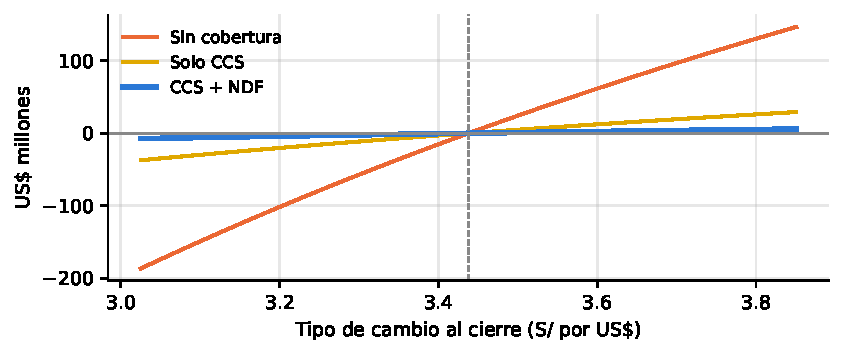
\includegraphics[width=0.8\linewidth]{f_e1_escenarios}
  \caption{E1: Resultado cambiario con y sin cobertura según el TC al cierre}\label{fig:e1}
  \fuente{\textcite{petroperu2026eeff}, Notas 3 y 14; \textcite{bcrpseries2026}. Elaboración propia.}
\end{figure}

\textbf{Escenarios.} Con la posición a la fecha de valorización (S/~\PosicionHoy\ millones al TC medio de
\SpotUSDPEN), una caída de 10\,\% del tipo de cambio (una apreciación del sol de \ApreciacionSolDiez) costaría
US\$~\EscSinCobMenosDiez\ millones sin cobertura y solo US\$~\EscConCobMenosDiez\ millones con el CCS y los NDF: la
sensibilidad cae en \ReduccionFX\ (Cuadro~\ref{tab:e1-escenarios} y Figura~\ref{fig:e1}). La pérdida sin cobertura
difiere de los US\$~\SensApreciacion\ millones de la sección~2 porque aquella parte del TC de cierre de 2025. A cambio, la Compañía renuncia a la ganancia si el sol se deprecia; el objetivo es
estabilizar resultados y flujos, no especular \parencite{stulz1996}.

\textbf{Registro contable.} Ambos derivados se pactan a valor cero y luego se miden a valor razonable: como activo si
el valor es favorable y como pasivo si no. Ante una caída instantánea de 10\,\% del TC, el CCS sería un activo de
US\$~\CCSValMenosDiez\ millones y el NDF uno de US\$~\NDFValMenosDiez\ millones; si el TC sube 10\,\%, serían pasivos
de US\$~\CCSValMasDiez\ y \NDFValMasDiez\ millones. Difieren algo de la compensación nominal del
Cuadro~\ref{tab:e1-posiciones}, porque el cupón del BN supera la curva y el NDF aún no vence: esa brecha es la
inefectividad esperada. El CCS se designa como cobertura de flujos de efectivo del préstamo
del BN: la parte efectiva va a otro resultado integral y se reclasifica cuando la diferencia de cambio del préstamo
afecta resultados. La relación debe documentarse sobre el cronograma contractual; sus fuentes de inefectividad son las
diferencias de cronograma, el CVA y el basis, que puede excluirse de la designación (NIIF~9, 6.5.16). El NDF no se
designa: cubre partidas monetarias ya reconocidas, cuya diferencia de cambio va a resultados por la NIC~21, y medido a
valor razonable con cambios en resultados la compensa en el mismo estado, sin contabilidad de coberturas \parencite{ifrs9}.

\subsection{Estrategia 2: swap y collar de costo cero sobre WTI para el inventario de crudo}

\textbf{Diseño.} Lo que está expuesto es el desfase de precios: el crudo se paga al precio de su embarque y los
productos se venden por paridad de importación semanas después, así que el inventario pierde valor si el precio cae
antes de trasladarse a ventas. Las compras aún sin precio no suman exposición, porque las ventas que financiarán
fijarán su precio en el mismo mercado. Con compras de \ComprasMBDC\ MBDC, las \InvCrudoMbl\ MBL rotan en unos
\RotacionDias\ días. Por eso la cobertura se arma en \NCapas\ \textbf{capas mensuales}: un tercio del volumen en los
contratos de noviembre, diciembre y enero, cada capa sobre el inventario que se venderá ese mes. Se cubre el
\CoberturaCrudoPct\ (\InvCubiertoMMbl\ MMbl), tope de la política propuesta, del inventario al cierre de 2025, que al
WTI de US\$~\WTISpot/bl vale US\$~\InvValorHoy\ millones. No se cubre el inventario de productos
(US\$~\InvRefinadosUSD\ millones), cuyo precio ya sigue la paridad con menor desfase. Se usan instrumentos OTC, porque
los futuros NYMEX exigen márgenes diarios. El \RepartoSwap\ del volumen va a (a) un \textbf{swap de WTI} con
liquidaciones mensuales a US\$~\SwapPrecio/bl (promedio de los futuros de noviembre a enero), para cargamentos con
margen ya definido; el resto, a (b) un \textbf{collar de costo cero} por capa: un put comprado al \PutPctFwd\ del
futuro de cada mes (US\$~\CollarPutsCapas) financiado con un call vendido (US\$~\CollarCallsCapas). Las opciones
vencen en \PlazoDiasCapas\ días y se valorizan con el modelo de \textcite{black1976}:
\begin{equation}
  P = e^{-rT}\left[K\,N(-d_2) - F\,N(-d_1)\right],\qquad
  d_1 = \frac{\ln(F/K) + \sigma^2T/2}{\sigma\sqrt{T}},\quad d_2 = d_1 - \sigma\sqrt{T}.
\end{equation}

\begin{table}[t]\centering\small
\caption{E2: Parámetros y valorización del collar sobre WTI al \FechaValorizacion}\label{tab:e2-param}
\renewcommand{\arraystretch}{1.0}
\newcommand{\grupo}[1]{\rowcolor{gray!12}\multicolumn{3}{l}{\textit{#1}}\\}
\begin{tabularx}{\linewidth}{>{\raggedright\arraybackslash}p{5.3cm} r >{\raggedright\arraybackslash}X}
\toprule
\textbf{Parámetro} & \textbf{Valor} & \textbf{Fuente / supuesto} \\
\midrule
\grupo{Insumos de mercado}
Futuros $F$ nov / dic / ene (US\$/bl) & \WTIFutUno\ / \WTIFutDos\ / \WTIFut & NYMEX CL, 28-sep-2026 \\
Volatilidad implícita, $\sigma$ & \VolCrudo & Índice OVX; realizada a un año: \VolRealCL \\
Plazo al vencimiento, $T$ (días) & \PlazoDiasCapas & NYMEX: 7 días hábiles antes del 26 del mes previo \\
Tasa libre de riesgo, $r$ & \RUSDCont & SOFR, capitalización continua \\
\grupo{Estructura del collar (costo cero, por capa nov / dic / ene)}
Volumen cubierto: total / en collar (MMbl) & \InvCubiertoMMbl\ / \InvCollarMMbl & \CoberturaCrudoPct\ del inventario; \ContratosEquiv\ contratos (1:1) \\
Put comprado: strike (US\$/bl) & \CollarPutsCapas & \PutPctFwd\ de $F$ \\
Put comprado: prima media (US\$/bl) & \PrimaPut & \textcite{black1976}; delta medio $-$\DeltaPutAbs \\
Call vendido: strike (US\$/bl) & \CollarCallsCapas & Su prima iguala la del put: prima neta cero \\
\grupo{Resultado del inventario total si el WTI cae 30\,\% (US\$ MM)}
Sin cobertura & (\PerdidaSinCobTreinta) & Valor del inventario a mercado \\
Solo collar & (\PerdidaMaxCollar) & Piso del put sobre lo cubierto \\
\textbf{Propuesta: swap + collar} & \textbf{(\PerdidaMaxMixto)} & Solo put sobre el \CoberturaCrudoPct: US\$~\CostoPutTotal\ MM \\
\bottomrule
\end{tabularx}
\fuente{\textcite{petroperu2026eeff}, Nota 10; \textcite{yahoo2026cl}; \textcite{fred2026}; \textcite{bluegamma2026}. Elaboración propia con el modelo de \textcite{black1976}.}
\end{table}

% ARCHIVO GENERADO — NO EDITAR A MANO
\begin{table}[htbp]\centering\small
\caption{E2: Resultado sobre el inventario de crudo al vencimiento (US\$ millones)}\label{tab:e2-escenarios}
\begin{tabular}{lrrrrrrrr}
\toprule
 & \textbf{-30\%} & \textbf{-20\%} & \textbf{-10\%} & \textbf{$=F$} & \textbf{0\%} & \textbf{+10\%} & \textbf{+20\%} & \textbf{+30\%} \\
\midrule
WTI (US\$/bbl) & 64.8 & 74.1 & 83.3 & 86.5 & 92.6 & 101.9 & 111.1 & 120.4 \\
Sin cobertura & (80.6) & (53.7) & (26.9) & (17.6) & 0.0 & 26.9 & 53.7 & 80.6 \\
Swap (venta a 89.38) & (9.3) & (9.3) & (9.3) & (9.3) & (9.3) & (9.3) & (9.3) & (9.3) \\
Collar 77.90 / 98.08 & (42.6) & (42.6) & (26.9) & (17.6) & 0.0 & 15.9 & 15.9 & 15.9 \\
Solo put (prima pagada) & (57.0) & (57.0) & (41.2) & (31.9) & (14.4) & 12.5 & 39.4 & 66.2 \\
Propuesta: 50\% swap + 50\% collar & (26.0) & (26.0) & (18.1) & (13.5) & (4.7) & 3.3 & 3.3 & 3.3 \\
\bottomrule
\end{tabular}
\fuente{PETROPERÚ, EEFF auditados al 31.12.2025 (Gaveglio, Aparicio y Asociados, 2026), Nota 10; NYMEX CL vía Yahoo Finance; CBOE OVX vía FRED (28-sep-2026). Elaboración propia. Variación del WTI respecto del precio del 28-sep-2026. Signo negativo = pérdida.}
\end{table}


\begin{figure}[t]\centering
  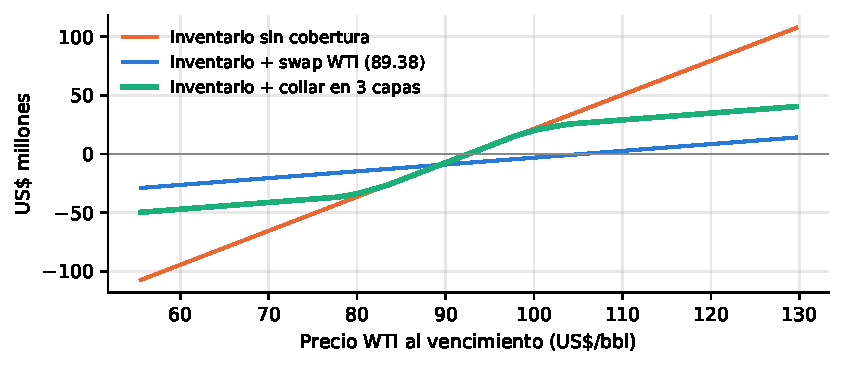
\includegraphics[width=0.8\linewidth]{f_e2_payoff}
  \caption{E2: Perfil de resultados de la cobertura del inventario de crudo}\label{fig:e2}
  \fuente{\textcite{petroperu2026eeff}, Nota 10; \textcite{yahoo2026cl}; \textcite{fred2026}. Elaboración propia.}
\end{figure}

\textbf{Escenarios.} El mercado presenta una fuerte \emph{backwardation}: el futuro de enero está \Backwardation\
por debajo del contrato frente. El modelo de costo de acarreo, $F=S\,e^{(r-y)T}$, lo explica con un rendimiento de
conveniencia neto implícito de \ConvenienciaImplicita\ anual entre ambos contratos, muy superior a la tasa libre de
riesgo (\RUSDCont): en plena crisis de oferta el mercado paga por tener crudo disponible hoy \parencite{hull2022}.
Por eso toda venta a plazo fija un precio menor que el actual: sobre su volumen, el swap elimina la variabilidad a
cambio de US\$~\CostoSwap\ millones menos que el precio de hoy, pero su costo esperado frente al forward, que el mercado
ya descuenta, es nulo. Pero si el WTI converge al futuro (columna
$=F$ del Cuadro~\ref{tab:e2-escenarios}), el inventario sin cobertura pierde US\$~\PerdidaSinCobForward\ millones, más
que el swap. Si el WTI cae 30\,\%, el inventario pierde US\$~\PerdidaSinCobTreinta\ millones sin cobertura y
US\$~\PerdidaMaxCollar\ millones con el collar, que conserva la ganancia hasta el strike del call de cada capa y no
requiere una prima que la caja no puede financiar; comprar solo el put sobre todo lo cubierto
costaría US\$~\CostoPutTotal\ millones. En ese escenario la combinación propuesta reduce la pérdida a
US\$~\PerdidaMaxMixto\ millones. Si el WTI sube, la Compañía renuncia a parte de la ganancia (con un alza de
30\,\% gana US\$~\GananciaMaxMixto\ millones); aun así conviene, porque protege la caja de una empresa sin margen para absorber otra caída como la de 2025
\parencite{froot1993}. El OVX coincide con la volatilidad realizada del CL a un año (\VolRealCL; el \VolHistWTI\ de la sección~2 usa
promedios mensuales); con $\sigma=$~\VolSensBaja\ el call de enero apenas cambiaría (US\$~\CollarCallVolBaja), pero el
\emph{skew}, no modelado, obliga a confirmar los strikes con bancos.

El principal riesgo residual es el de base: PETROPERÚ compra crudos referidos al Brent, cuyo diferencial con el WTI
es hoy de US\$~\BrentWTI/bl, y crudos pesados con descuento. El ratio de mínima varianza $h^*=\rho\,\sigma_S/\sigma_F$
del Brent frente al futuro CL es \RatioHBrent, con una efectividad $\rho^2$ de \EfectividadBrent\ (\SemanasH\
semanas; para el WTI de Cushing: \RatioH\ y \EfectividadWTI) \parencite{hull2022}. Si la partida fuera el Brent, el
nocional subiría a \ContratosHBrent\ contratos y una quinta parte de la varianza quedaría sin cubrir. Se mantiene el
WTI porque los precios de venta locales siguen la paridad de importación sobre el WTI más spreads (Nota~11(viii),
p.~70), lo que lo hace un componente de riesgo identificable (NIIF~9, 6.3.7); los swaps sobre Brent (ICE) son la
alternativa si la serie interna de costos de compra se ajusta mejor a ese marcador.

\medskip\noindent
\begin{minipage}[t]{0.5\linewidth}\footnotesize\setlength{\tabcolsep}{2.5pt}% ARCHIVO GENERADO — NO EDITAR A MANO
\centering
\captionof{table}{E2: posiciones en barriles (MM)}\label{tab:e2-posiciones}
\begin{tabular}{lrr}
\toprule
 & \textbf{MMbl} & \textbf{WTI $-10$\,\% (US\$)} \\
\midrule
Físico: inventario de crudo & 2.90 & (26.86) \\
Swap (vende a precio fijo) & (1.16) & 10.75 \\
Collar (equivalente delta) & (0.62) & 5.75 \\
Global (físico + derivados) & 1.12 & (10.37) \\
\bottomrule
\end{tabular}
\fuente{\textcite{petroperu2026eeff}, Nota 10; NYMEX CL vía Yahoo Finance; CBOE OVX vía FRED (28-sep-2026). Elaboración propia. Positivo = largo en crudo. Collar: delta medio de las capas. Efecto lineal de una caída de 10 \% del WTI.}
\end{minipage}\hfill
\begin{minipage}[t]{0.47\linewidth}\textbf{Demostración de la cobertura.} Sobre su volumen (\InvSwapMMbl\ MMbl),
inventario y swap suman $-$US\$~\CostoSwap\ millones en cualquier escenario: lo que pierde el crudo lo gana el swap.
En barriles, los derivados reducen la posición larga de \InvCrudoMMbl\ a \PosGlobalMMbl\ MMbl equivalentes
(\PosGlobalPct): queda el 20\,\% abierto y la zona entre strikes del collar.\end{minipage}
\medskip

\textbf{Registro contable.} El swap y el collar se pactan a valor cero. Ante una caída instantánea de 10\,\% de la
curva de futuros, el collar sería un activo de US\$~\CollarValMenosDiez\ millones y el swap uno de
US\$~\SwapValDiez\ millones; con un alza de 10\,\%, serían pasivos de US\$~\CollarValMasDiez\ y \SwapValDiez\
millones. Cada capa se designa como cobertura de valor razonable del inventario de su mes: el ajuste por el riesgo
cubierto modifica el costo del inventario y va a resultados junto con el derivado. Al venderse la capa, la relación se
discontinúa (NIIF~9, 6.5.6) y se designa la siguiente. El Cuadro~\ref{tab:e2-escenarios} es económico: la pérdida
contable depende del costo y del valor neto de realización (NIC~2), no del spot \parencite{ifrs9}.
       % 2.4 p  [4.0]
% Comparación de estrategias, riesgo residual, liquidez (colateral), tasa (no recomendada hoy), condiciones y límites.
\section{Análisis comparativo e implementación}

Ambas estrategias reducen el riesgo en la magnitud que importa y no exigen pago inicial. Lo que puede impedir
ejecutarlas no es su costo, sino el colateral que pediría el banco. El Cuadro~\ref{tab:comparacion} las compara con
los mismos criterios.

\begin{table}[htbp]\centering\small
\caption{Comparación: E1 y E2 reducen el riesgo sin costo inicial; el límite es el colateral}\label{tab:comparacion}
\renewcommand{\arraystretch}{1.25}
\newcommand{\filasep}{\arrayrulecolor{gray!45}\specialrule{0.3pt}{1pt}{1pt}\arrayrulecolor{black}}
\newcommand{\encab}[2]{\textbf{#1}\newline #2}
\begin{tabularx}{\linewidth}{>{\raggedright\arraybackslash\bfseries}p{2.3cm}
    >{\raggedright\arraybackslash}X
    >{\raggedright\arraybackslash}X
    >{\raggedright\arraybackslash}X}
\toprule
\normalfont\textbf{Criterio}
  & \cellcolor{prioAlta}\encab{E1: tipo de cambio}{CCS + NDF}
  & \cellcolor{prioAlta}\encab{E2: precio del crudo}{Swap + collar WTI}
  & \cellcolor{prioMedia}\encab{Tasa de interés}{\textit{No recomendada hoy}} \\
\midrule
Exposición cubierta & \CoberturaFX\ de la posición en S/
  & \InvCubiertoMMbl\ MMbl, \CoberturaCrudoPct\ del inventario \newline (US\$~\InvCubiertoValor\ MM)
  & Tasa base de la refinanciación del CESCE (US\$~\CESCESaldo\ MM) \\ \filasep
Reducción del riesgo \newline {\normalfont (US\$ MM)}
  & Pérdida si el TC cae 10\,\%: \newline Sin cobertura: (\EscSinCobMenosDiez) \newline Con cobertura: (\EscConCobMenosDiez)
  & Pérdida si el WTI cae 30\,\%: \newline Sin cobertura: (\PerdidaSinCobTreinta) \newline Con cobertura: (\PerdidaMaxMixto)
  & Baja: no cubre el spread de crédito \\ \filasep
Costo inicial & Cero; CVA de \CCSCVApb~pb en la tasa & Cero (swap y collar) & Cero (swap de inicio diferido) \\ \filasep
Costo económico & Diferencial implícito del NDF: \NDFCostoAnual\ anual
  & Swap: US\$~\CostoSwap\ MM frente al spot (nulo frente al forward)
  & Pagos si la tasa baja \\ \filasep
Colateral con umbral cero \newline {\normalfont (US\$ MM)} & \ColateralTC\ si el TC sube 10\,\% & \ColateralWTI\ si el WTI sube 30\,\% & Bajo \\ \filasep
Tratamiento NIIF~9 & CCS: flujos de efectivo (ORI); NDF: valor razonable en resultados
  & Valor razonable del inventario existente; se redesigna al rotar
  & Flujos de efectivo, solo si la refinanciación es altamente probable \\
\bottomrule
\end{tabularx}
\fuente{Cuadros~\ref{tab:e1-param} a \ref{tab:e2-escenarios}; \textcite{ifrs9}. Elaboración propia. El inventario cubierto se valora al WTI de la fecha de valorización; al cierre de 2025 el inventario de crudo valía US\$~\InvCrudoUSD\ MM (Cuadro~\ref{tab:matriz}).}
\end{table}

\textbf{Riesgo residual.} El VaR al 95\,\% es la pérdida que solo se supera en uno de cada veinte casos. Al
vencimiento de cada cobertura, baja de US\$~\VaRFXSin\ a \VaRFXCon\ millones en la E1 y de \VaRCrudoSin\ a
\VaRCrudoCon\ millones en la E2 (Cuadro~\ref{tab:var}). La E2 conserva más riesgo porque deja abierto el 20\,\% del
inventario y la zona entre los strikes del collar.

\textbf{Liquidez: la restricción que decide.} Los derivados OTC no tienen márgenes de bolsa, pero el banco pedirá
colateral a una contraparte B-/Caa1. El \emph{umbral} del anexo CSA es la pérdida que el banco tolera antes de pedir
garantías en efectivo; se supone umbral cero, el caso más exigente. Un choque instantáneo conjunto (TC $+10$\,\% y
WTI $+30$\,\%) exigiría US\$~\ColateralConjunto\ millones, pero el CCS vive 27 meses: lo relevante es la
exposición potencial futura (PFE) al 99\,\% en toda su vida. Con el NDF y la E2 (correlación TC--WTI de \CorrTCWTI)
llega a US\$~\PFENoventaNueve\ millones, frente a US\$~\LineasLibres\ millones de líneas libres
(Cuadro~\ref{tab:colateral}); el préstamo puente (US\$~\PrestamoPuente\ millones) tiene otro destino. La ejecución
exige un umbral total de al menos US\$~\UmbralNecesario\ millones (unos \UmbralPorBanco\ por banco, con
\NContrapartes), que deja libre el \ColchonLineas\ de las líneas, o la garantía del Estado; sin ello, la cobertura
agravaría el riesgo de liquidez que busca mitigar \parencite{moodys2026petroperu}.

\medskip\noindent
\begin{minipage}[t]{0.42\linewidth}\footnotesize\setlength{\tabcolsep}{2.5pt}% ARCHIVO GENERADO — NO EDITAR A MANO
\centering
\captionof{table}{VaR al 95\,\% al vencimiento de la cobertura (US\$ MM)}\label{tab:var}
\begin{tabular}{lrrr}
\toprule
 & \textbf{Sin cob.} & \textbf{Con cob.} & \textbf{Reducción} \\
\midrule
E1 (TC) & 78.5 & 3.1 & 96\% \\
E2 (crudo) & 93.3 & 36.5 & 61\% \\
\bottomrule
\end{tabular}
\fuente{BCRP, series estadísticas; NYMEX CL vía Yahoo Finance; CBOE OVX vía FRED (28-sep-2026). Volatilidad realizada de un año. Elaboración propia. Horizonte: 91 días (E1) y vencimiento de las opciones (E2). La E2 incluye el 20 \% no cubierto.}
\end{minipage}\hfill
\begin{minipage}[t]{0.55\linewidth}\footnotesize\setlength{\tabcolsep}{2.5pt}% ARCHIVO GENERADO — NO EDITAR A MANO
\centering
\captionof{table}{Colateral exigible con umbral cero (US\$ MM)}\label{tab:colateral}
\begin{tabular}{lrrrr}
\toprule
 & \textbf{E1} & \textbf{E2} & \textbf{Colat.} & \textbf{Déficit} \\
\midrule
TC $+10$\,\% & 121.6 & 0.0 & 121.6 & 99.4 \\
WTI $+30$\,\% & 0.4 & 51.8 & 52.2 & 30.0 \\
TC $+10$\,\% y WTI $+30$\,\% & 121.6 & 51.8 & 173.4 & 151.2 \\
PFE 95\,\% & 108.3 & 97.5 & 168.9 & 146.7 \\
PFE 99\,\% & 151.4 & 157.8 & 253.6 & 231.4 \\
\bottomrule
\end{tabular}
\fuente{\textcite{petroperu2026eeff}, Nota 3.1(c); BCRP, series estadísticas; NYMEX CL vía Yahoo Finance; CBOE OVX vía FRED (28-sep-2026). Elaboración propia. E1 y E2: pasivo de los derivados, a TC medio. Choques: instantáneos. PFE: pico en la vida del CCS más NDF a 91 días (E1) y programa rodante a su plazo (E2), lognormal con volatilidad realizada; E1 y E2 agregadas con correlación TC--WTI de 0.35. Déficit: colateral menos líneas libres (US\$ 22.2 MM).}
\end{minipage}
\medskip

\textbf{Plan B si el banco no concede el umbral.} (a) Escalonar: contratar primero el 50\,\% del CCS, con lo que el
colateral ante un TC $+10$\,\% baja a US\$~\ColateralTCMitad\ millones. (b) Comprar opciones, que solo exigen prima y
ningún colateral; el put de WTI sobre el \CoberturaCrudoPct\ cuesta US\$~\CostoPutTotal\ millones, por lo que se
limitaría al tramo más expuesto. (c) Pactar un umbral escalonado según la calificación y un reajuste semanal del
colateral, en lugar de diario. (d) Obtener la garantía del Estado sobre la línea de derivados.

\textbf{Riesgo de tasa: no se recomienda cubrirlo hoy.} La deuda de largo plazo ya es fija; pasarla a variable añadiría riesgo sin
bajar el costo de crédito, que lo domina el spread. Queda como opción un swap de inicio diferido para la
refinanciación del CESCE (tasa de \FwdSwapRate\ con pago anual), solo cuando esa refinanciación sea altamente probable
(NIIF~9, 6.3.3). Hoy no lo es, por el incumplimiento del covenant.

\textbf{Condiciones de implementación.} (i) El Directorio aprueba una Política de Cobertura con límites (\LimiteFX\
de la posición en soles y \LimiteCrudo\ del inventario de crudo), prohibición expresa de especular y métricas
mensuales. (ii) Se firman contratos ISDA con anexo CSA y un umbral de al menos US\$~\UmbralNecesario\ millones, o se
aplica el plan B, con período de reposición del colateral y monto mínimo de transferencia. Como el covenant del
CESCE ya está incumplido, el incumplimiento cruzado del ISDA (§5(a)(vi)) se limita a deudas efectivamente aceleradas
(\emph{cross-acceleration}), con umbral alto y dispensa expresa para el CESCE; sin ella, no se firma. Se negocia además que la rebaja de calificación, la opinión con salvedades o la incertidumbre de
empresa en marcha no causen el cierre inmediato sin un período de cura. También una cláusula de prepago: si el BN
prepaga el préstamo, el CCS debe poder cancelarse a valor de mercado. (iii) Antes de pactar, la Gerencia Legal opina y
se obtiene la autorización que exija el régimen de endeudamiento y tesorería de una empresa del Estado. Se evalúa si
los compromisos contingentes que el D.U.~\DUCrisis\ autoriza al MINEM (hasta US\$~\DUCrisisMonto\ millones, Nota~1,
p.~25) pueden respaldar las líneas de derivados. (iv) Las coberturas se documentan según la NIIF~9 y se revelan según la NIIF~7, ¶21A--24G
\parencite{ifrs9}; los swaps con Citibank entran a la política. (v) Se separan funciones: Finanzas contrata; Riesgos controla límites y verifica de forma independiente los
precios de los bancos; Contabilidad registra \parencite{humala2026}. La política fija límites por contraparte y de pérdida, y Riesgos
aprueba los modelos; con insumos proxy y el CVA, el nivel de valor razonable (2 o 3; NIIF~13, ¶73) se determina por
instrumento. El reporte
regulatorio se coordina con cada banco.

\textbf{Supuestos que limitan el resultado.} Las cifras son indicativas. El cronograma del BN es inferido (tasa
del CCS entre \CCSTasaMin\ y \CCSTasaMax). La posición en soles distinta del BN y el inventario son de diciembre de
2025: si cambiaron, cambian los nocionales (nunca por encima de la exposición al pactar), no el diseño. La curva soberana y el OVX sustituyen a la curva swap y a la
superficie de volatilidad, que no son públicas. Antes de pactar se requieren el cronograma contractual, la posición
actualizada y cotizaciones ejecutables de al menos tres bancos (no BlueGamma ni Yahoo Finance).
          % 2.8 p  [4.0]  (+ Material de apoyo [3.5] repartido en todo el texto)
% [1.5 pts] ~0.6 páginas. Recomendación concreta y accionable; no repetir el análisis.
\section{Conclusiones y recomendaciones}
\begin{itemize}
  \item Se recomienda cubrir con derivados los dos riesgos de mercado que hoy se asumen sin cobertura y que, con
  utilidad bruta casi nula y liquidez restringida, comprometen la continuidad operativa: la posición pasiva neta de
  S/~\PenNetoAbs\ millones, sin amortizaciones del BN hasta 2027, y el inventario de crudo, expuesto a un WTI que cayó
  \WTICaidaVeinticinco\ en 2025 y hoy cotiza en US\$~\WTISpot/bl con una volatilidad implícita de \VolCrudo.
  \item \textbf{Estrategia 1:} el CCS amortizable sobre el préstamo del BN, pagando en dólares al \CCSTasaAllIn\ (con
  CVA), junto con NDF de compra de soles, cubre el \CoberturaFX\ de la exposición en soles y reduce la pérdida ante
  una caída de 10\,\% del tipo de cambio de US\$~\EscSinCobMenosDiez\ millones a US\$~\EscConCobMenosDiez\ millones, sin
  costo inicial y con contabilidad de coberturas para el CCS; su costo es el diferencial de tasas (\NDFCostoAnual\ anual).
  \item \textbf{Estrategia 2:} cubrir el \CoberturaCrudoPct\ del inventario de crudo, por partes iguales con un swap de WTI a
  US\$~\SwapPrecio/bl y con collares de costo cero en tres capas mensuales (puts al \PutPctFwd\ de cada futuro), reduce la
  pérdida ante una caída de 30\,\% del WTI a US\$~\PerdidaMaxMixto\ millones (frente a US\$~\PerdidaSinCobTreinta\
  millones) sin pagar prima.
  \item La restricción de liquidez obliga a preferir instrumentos OTC sin costo inicial en lugar de futuros con
  márgenes diarios; aun así, en un estrés conjunto el colateral llegaría a US\$~\ColateralConjunto\ millones, por lo que
  la ejecución se condiciona a un umbral CSA de al menos US\$~\UmbralNecesario\ millones o a la garantía del Estado. Para el riesgo de tasa conviene esperar al diseño de la refinanciación
  y evaluar entonces un swap de inicio diferido, solo si la refinanciación es altamente probable.
  \item Se recomienda a la Gerencia General: (1) presentar la Política de Cobertura al Directorio; (2) iniciar la
  negociación ISDA/CSA con al menos tres bancos; (3) obtener la opinión legal y gestionar el respaldo del Estado (MINEM, D.U.~\DUCrisis) para las líneas de
  derivados; y (4) ejecutar primero el CCS, que cubre el riesgo de mayor impacto, una vez firmado el CSA con el umbral
  requerido.
\end{itemize}
      % 0.6 p  [1.5]

\printbibliography[heading=bibintoc,title={Referencias}]  % 0.6 p [1.5]

\end{document}
